\documentclass[10pt]{amsart}
%\include{amsmath}
\usepackage[margin=1.5in]{geometry}
\usepackage{mathtools}
\usepackage{bbm}
\usepackage{amsmath}  
\usepackage{amssymb}  % gives you \mathbb{} font
\usepackage{dsfont}	% gives you \mathds{} font
\usepackage{bm} %gives bold font in equations

%                   Math Blackboard Bold Symbols

\newcommand\Cb{\mathds{C}}
\newcommand\Eb{\mathds{E}}
\newcommand\Fb{\mathds{F}}
\newcommand\Gb{\mathds{G}}
\newcommand\Ib{\mathds{I}}
\newcommand\Pb{\mathds{P}}
\newcommand\Qb{\mathds{Q}}
\newcommand\Rb{\mathds{R}}
%\newcommand\Zb{\mathds{Z}}
\newcommand\Nb{\mathds{N}}
\newcommand\Vb{\mathds{V}}
\newcommand\Ub{\mathds{U}}

\usepackage[shortlabels]{enumitem}
\usepackage{amssymb}
\usepackage{bbm}
\usepackage{bm}
\usepackage{cancel}
\usepackage{graphicx,subfig}

\graphicspath{ {./images/} }

\newcommand{\D}{\mathrm{d}}
\DeclareMathOperator{\E}{e}
\DeclareMathOperator{\I}{i}


\begin{document}

\noindent
\text{Hunter Lybbert} \\
\text{Student ID: 2426454} \\
\text{12-13-24} \\
\text{AMATH 561}
\title{Final Exam}
\maketitle

{\it Note: Submit electronically to Canvas.}
\\

\noindent {\bf Directions:} You are to work alone on this exam. You may use everything that is on the course website (lectures, homework solutions) and Lorig lecture notes. You may {\it not} use the internet, or discuss the exam with others. You may use Mathematica, or any other computational tool you find helpful. Good luck! 
\\

\noindent {\bf 1.} Consider two continuous time Markov chains $X=(X_t)_{t\geq0}$ and $Y=(Y_t)_{t\geq0}$ that evolve independently on the same state space $S=\{1,2,...,N+1\}$. After $X$ arrives in any state, it remains there for a random amount of time, which is exponentially distributed with parameter $\mu$. When $X$ leaves a state, it jumps to any other state with equal probability (i.e. the probability that $X$ jumps from $i$ to $j$ is $1/N$ for $j \neq i$). After $Y$ arrives in a state, it remains there for a random amount of time, which is exponentially distributed with parameter $\lambda$. When $Y$ leaves a state, it can jump to any other state with equal probability. 
\\

\noindent {\bf (a)} Write the generator $G$ of $X$. \\

\noindent
\textit{Solution:} \\
As the Markov Chain $X$ is described, given a small amount of time $\Delta t$ we can say 
$$
p_{\Delta t}(i,j) = P(X_{t + \Delta t} = j | X_t = i) = \frac 1 N, \quad \text{ for } i \neq j.
$$
Recall that we have
\begin{align*}
p_{\Delta t}(i, j) &= g(i, j) \Delta t + \mathcal O(\Delta t)
\end{align*}
and
\begin{align*}
p_{\Delta t}(i, i) &= 1 + g(i, i) \Delta t + \mathcal O(\Delta t) \\
- 1 + p_{\Delta t}(i, i) &= g(i, i) \Delta t + \mathcal O(\Delta t) \\
p_{\Delta t}(i, i) - 1 &= - g(i, i) \Delta t - \mathcal O(\Delta t).
\end{align*}
Furthermore, with the state space $S = \{1, 2, ..., N + 1\}$, the generator can be denoted as
\begin{align*}
\bm G_X = 
\begin{bmatrix}
- \mu & 1/N & 1/N & \dots & 1/N \\
1/N & - \mu & 1/N & \dots & 1/N \\
1/N & 1/N & - \mu & \dots & 1/N \\
\vdots & \vdots & \vdots & \ddots & \vdots \\
1/N & 1/N & 1/N & \dots & - \mu \\
\end{bmatrix}.
\end{align*}
\textbf{TODO:}
Moreover, I am speculating that $\mu = 1 - \frac 1 N$, but my only hesitation is that we don't necessarily know that $p_{\Delta t}(i,i) = 1/N$ as well. \\
\qed \\


\noindent {\bf (b)} Now, consider a Markov chain $Z=(Z_t)_{t\geq0}$, defined as follows:
$$Z_t=\mathbbm{1}_{\{X_t=Y_t\}}+2 \mathbbm{1}_{\{X_t\neq Y_t\}}.$$
Write the generator $H$ of $Z$. \\

\noindent
\textit{Solution: } \\
Notice that there are only two states for the Markov chain $Z$ and they are $S_Z = \{1, 2\}$.
The nature of defining it by these indicator functions is equivalent to saying
$$
Z_t = \begin{cases}
1 \quad \text{ if } X_t = Y_t\\
2 \quad \text{ if } X_t \neq Y_t\\
\end{cases}
$$
We now need to think through the possible ways this occurs.
Suppose at time $s$ (which could be $0$) we have $Z_s = 2$ meaning $X_s \neq Y_s$. \\

\noindent
\textbf{Case 1: $Z$ goes from 2 to 1} \\
For notational assistance suppose $X_s = i$ and $Y_s = j$ where $i \neq j$.
The means by which $Z_{s + t} = 1$ are the following scenarios ( I recognize the short coming of my notation in this interim section while I am still thinking through the way these probabilities will work together)
\begin{enumerate}
\item $X$ does not change states but $Y$ changes to state $i$.
That is $X_{s + t} = i$ and $Y_{s + t} = i$.
This can occur w.p. (using the fact that $X$ and $Y$ are independent Markov chains)
\begin{align*}
P(Z_{s + t} = 1 | Z_s = 2)
	&= P(X_{s + t} = i,Y_{s + t} = i | X_s = i,Y_s = j) \\
	&= P(X_{s + t} = i| X_s = i)P(Y_{s + t} = i | Y_s = j) \\
	&= p_X(t,i;s,i) p_Y(t,i;s,j) \\
	&= \mu\E^{-\mu(t + s)} \frac 1 N.
\end{align*}
\item The opposite outcome where $Y$ does not change states but $X$ changes to state $j$.
That is $X_{s + t} = j$ and $Y_{s + t} = j$.
This can occur w.p. (using the fact that $X$ and $Y$ are independent Markov chains)
\begin{align*}
P(Z_{s + t} = 1 | Z_s = 2)
	&= P(X_{s + t} = j,Y_{s + t} = j | X_s = i,Y_s = j) \\
	&= P(X_{s + t} = j| X_s = i)P(Y_{s + t} = j | Y_s = j) \\
	&= p_X(t,j;s,i)p_Y(t,j;s,j) \\
	&= \frac 1 N \lambda\E^{-\lambda(t + s)}.
\end{align*}
\item Lastly, it is possible that $X$ and $Y$ both change to the same new state $k$.
That is $X_{s + t} = k$ and $Y_{s + t} = k$.
This can occur w.p. (using the fact that $X$ and $Y$ are independent Markov chains)
\begin{align*}
P(Z_{s + t} = 1 | Z_s = 2)
	&= P(X_{s + t} = k,Y_{s + t} = k | X_s = i,Y_s = j) \\
	&= P(X_{s + t} = k| X_s = i)P(Y_{s + t} = k | Y_s = j) \\
	&= p_X(t,k;s,i)p_Y(t,k;s,j) \\
	&= \frac 1 N \frac 1 N \\
	&= \frac 1 {N^2}.
\end{align*}
\end{enumerate}
Therefore in it's totality 
$$
P(Z_{s + t} = 1 | Z_s = 2) = \mu\E^{-\mu(t + s)} \frac 1 N + \frac 1 N \lambda\E^{-\lambda(t + s)} + \frac 1 {N^2}
$$

\noindent
\textbf{Case 2: $Z$ goes from 1 to 1} \\
If $Z_s = 1$, then $X_s = Y_s = i$, for some $i \in S$.
The means by which $Z_{s + t} = 1$ or persists in this state are the following scenarios ( I recognize the short coming of my notation in this interim section while I am still thinking through the way these probabilities will work together)
\begin{enumerate}
\item $X$ and $Y$ do not change states and remain at $i$.
This can occur w.p. (using the fact that $X$ and $Y$ are independent Markov chains)
\begin{align*}
P(Z_{s + t} = 1 | Z_s = 1)
	&= P(X_{s + t} = i,Y_{s + t} = i | X_s = i,Y_s = i) \\
	&= P(X_{s + t} = i| X_s = i)P(Y_{s + t} = i | Y_s = i) \\
	&= p_X(t,i;s,i) p_Y(t,i;s,i) \\
	&= \mu\E^{-\mu(t + s)} \lambda\E^{-\lambda(t + s)}.
\end{align*}
\item Additionally, it is possible that $X$ and $Y$ both change to the same new state $k$.
That is $X_{s + t} = k$ and $Y_{s + t} = k$.
This can occur w.p. (using the fact that $X$ and $Y$ are independent Markov chains)
\begin{align*}
P(Z_{s + t} = 1 | Z_s = 1)
	&= P(X_{s + t} = k,Y_{s + t} = k | X_s = i,Y_s = i) \\
	&= P(X_{s + t} = k| X_s = i)P(Y_{s + t} = k | Y_s = i) \\
	&= p_X(t,k;s,i)p_Y(t,k;s,i) \\
	&= \frac 1 N \frac 1 N \\
	&= \frac 1 {N^2}.
\end{align*}
\end{enumerate}
Therefore in it's totality 
$$
P(Z_{s + t} = 1 | Z_s = 1) = \mu\E^{-\mu(t + s)} \lambda\E^{-\lambda(t + s)} + \frac 1 {N^2}
$$

\noindent
\textbf{Case 3: $Z$ goes from 1 to 2} \\
If $Z_s = 1$, then $X_s = Y_s = i$, for some $i \in S$.
The means by which $Z_{s + t} = 2$ are the following scenarios ( I recognize the short coming of my notation in this interim section while I am still thinking through the way these probabilities will work together)
\begin{enumerate}
\item $X$ does not change states but $Y$ changes to state $j$.
That is $X_{s + t} = i$ and $Y_{s + t} = j$.
This can occur w.p. (using the fact that $X$ and $Y$ are independent Markov chains)
\begin{align*}
P(Z_{s + t} = 2 | Z_s = 1)
	&= P(X_{s + t} = i,Y_{s + t} = j | X_s = i,Y_s = i) \\
	&= P(X_{s + t} = i| X_s = i)P(Y_{s + t} = j | Y_s = i) \\
	&= p_X(t,i;s,i) p_Y(t,j;s,i) \\
	&= \mu\E^{-\mu(t + s)} \frac 1 N.
\end{align*}
\item The opposite outcome where $Y$ does not change states but $X$ changes to state $j$.
That is $X_{s + t} = j$ and $Y_{s + t} = i$.
This can occur w.p. (using the fact that $X$ and $Y$ are independent Markov chains)
\begin{align*}
P(Z_{s + t} = 2 | Z_s = 1)
	&= P(X_{s + t} = j,Y_{s + t} = i | X_s = i,Y_s = i) \\
	&= P(X_{s + t} = j| X_s = i)P(Y_{s + t} = i | Y_s = i) \\
	&= p_X(t,j;s,i)p_Y(t,i;s,i) \\
	&= \frac 1 N \lambda\E^{-\lambda(t + s)}.
\end{align*}
\item Lastly, it is possible that $X$ and $Y$ both change to different new states $j$ and $k$, respectively (but without loss of generality).
That is $X_{s + t} = j$ and $Y_{s + t} = k$.
This can occur w.p. (using the fact that $X$ and $Y$ are independent Markov chains)
\begin{align*}
P(Z_{s + t} = 2 | Z_s = 1)
	&= P(X_{s + t} = j,Y_{s + t} = k | X_s = i,Y_s = i) \\
	&= P(X_{s + t} = j| X_s = i)P(Y_{s + t} = k | Y_s = i) \\
	&= p_X(t,j;s,i)p_Y(t,k;s,i) \\
	&= \frac 1 N \frac 1 N \\
	&= \frac 1 {N^2}.
\end{align*}
\end{enumerate}
Therefore in it's totality
$$
P(Z_{s + t} = 2 | Z_s = 1) = \mu\E^{-\mu(t + s)} \frac 1 N + \frac 1 N  \lambda\E^{-\lambda(t + s)} + \frac 1 {N^2}
$$

\noindent
\textbf{Case 4: $Z$ goes from 2 to 2} \\
If $Z_s = 2$, then $X_s = i$ and $Y_s = j$ where $i \neq j$ and $i, j \in S$.
The means by which $Z_{s + t} = 2$ are the following scenarios ( I recognize the short coming of my notation in this interim section while I am still thinking through the way these probabilities will work together)
\begin{enumerate}
\item $X$ does not change states but $Y$ changes to state $k$.
That is $X_{s + t} = i$ and $Y_{s + t} = k$.
This can occur w.p. (using the fact that $X$ and $Y$ are independent Markov chains)
\begin{align*}
P(Z_{s + t} = 2 | Z_s = 2)
	&= P(X_{s + t} = i,Y_{s + t} = k | X_s = i,Y_s = j) \\
	&= P(X_{s + t} = i| X_s = i)P(Y_{s + t} = k | Y_s = j) \\
	&= p_X(t,i;s,i) p_Y(t,k;s,j) \\
	&=  \mu\E^{-\mu(t + s)}  \frac 1 N.
\end{align*}
\item The opposite outcome where $Y$ does not change states but $X$ changes to state $k$.
That is $X_{s + t} = k$ and $Y_{s + t} = j$.
This can occur w.p. (using the fact that $X$ and $Y$ are independent Markov chains)
\begin{align*}
P(Z_{s + t} = 2 | Z_s = 2)
	&= P(X_{s + t} = k,Y_{s + t} = j | X_s = i,Y_s = j) \\
	&= P(X_{s + t} = k| X_s = i)P(Y_{s + t} = j | Y_s = j) \\
	&= p_X(t,k;s,i)p_Y(t,j;s,j) \\
	&= \frac 1 N  \lambda\E^{-\lambda(t + s)} .
\end{align*}
\item Lastly, it is possible that $X$ and $Y$ both change to different new states $k$ and $\ell$, respectively (but without loss of generality).
That is $X_{s + t} = k$ and $Y_{s + t} = \ell$ where $k \neq \ell$.
This can occur w.p. (using the fact that $X$ and $Y$ are independent Markov chains)
\begin{align*}
P(Z_{s + t} = 2 | Z_s = 2)
	&= P(X_{s + t} = k,Y_{s + t} = \ell | X_s = i,Y_s = j) \\
	&= P(X_{s + t} = k| X_s = i)P(Y_{s + t} = \ell | Y_s = j) \\
	&= p_X(t,k;s,i)p_Y(t,\ell;s,j) \\
	&= \frac 1 N \frac 1 N \\
	&= \frac 1 {N^2}.
\end{align*}
\item $X$ and $Y$ do not change states and remain at $i$ and $j$ respectively.
This can occur w.p. (using the fact that $X$ and $Y$ are independent Markov chains)
\begin{align*}
P(Z_{s + t} = 2 | Z_s = 2)
	&= P(X_{s + t} = i,Y_{s + t} = j | X_s = i,Y_s = j) \\
	&= P(X_{s + t} = i| X_s = i)P(Y_{s + t} = j | Y_s = j) \\
	&= p_X(t,i;s,i) p_Y(t,j;s,j) \\
	&= \mu\E^{-\mu(t + s)} \lambda\E^{-\lambda(t + s)}.
\end{align*}
\end{enumerate}
Therefore in it's totality
$$
P(Z_{s + t} = 2 | Z_s = 2) =  \mu\E^{-\mu(t + s)}  \frac 1 N + \frac 1 N  \lambda\E^{-\lambda(t + s)}  + \frac 1 {N^2} +  \mu\E^{-\mu(t + s)} \lambda\E^{-\lambda(t + s)} 
$$

\noindent
In summary we have the following transition probabilities
\begin{align*}
P(Z_{s + t} = 1 | Z_s = 1) &= p_Z(t,1;s,1) = \mu\E^{-\mu(t + s)} \lambda\E^{-\lambda(t + s)} + \frac 1 {N^2} \\
P(Z_{s + t} = 1 | Z_s = 2) &= p_Z(t,1;s,2) = \mu\E^{-\mu(t + s)} \frac 1 N + \frac 1 N \lambda\E^{-\lambda(t + s)} + \frac 1 {N^2} \\
P(Z_{s + t} = 2 | Z_s = 1) &= p_Z(t,2;s,1) = \mu\E^{-\mu(t + s)} \frac 1 N + \frac 1 N \lambda\E^{-\lambda(t + s)} + \frac 1 {N^2} \\
P(Z_{s + t} = 2 | Z_s = 2) &= p_Z(t,2;s,2) = \mu\E^{-\mu(t + s)} \frac 1 N + \frac 1 N \lambda\E^{-\lambda(t + s)} + \frac 1 {N^2} + \mu\E^{-\mu(t + s)} \lambda\E^{-\lambda(t + s)}.
\end{align*}

\noindent
Now how this information that I have deduced contributes to the generator, $\bm H$, for $Z$ is eluding me.
Let the generator be denoted as
\begin{align*}
\bm H_Z = 
\begin{bmatrix}
h(1,1), h(1,2) \\
h(2,1), h(2,2)
\end{bmatrix}.
\end{align*}
\textbf{TODO: Come back to this if I have new ideas.} \\
\qed \\


\noindent {\bf  (c)} Let ${\bm \mu}_t$ be the distribution of $Z_t$. Compute  ${\bm \mu}_t$ assuming $X_0=i$ and $Y_0=j$ where $i\neq j$. \\

\noindent
\textit{Solution:} \\
Now assuming $\bm \mu_t$ is the distribution of $Z_t$, I incidentally computed this information in the previous part.
The case we have here is when $s = 0$ and $X_0 = i$ and $Y_0 = j$ with $i \neq j$, in other terms $Z_0 = 2$.
Given the initial position we want to compute the distribution across the two possible states given this initial position.
Using what was computed in the previous part as $P(Z_{s + t} = 1 | Z_s = 2)$ and $P(Z_{s + t} = 2 | Z_s = 2)$, therefore
\begin{align*}
\bm \mu_t = \begin{bmatrix}
p_Z(t,1;0,2) \vspace{2 mm} \\ 
p_Z(t,2;0,2)
\end{bmatrix}^T
	= \begin{bmatrix}
\mu\E^{-\mu t } \frac 1 N + \frac 1 N \lambda\E^{-\lambda t} + \frac 1 {N^2} \vspace{2 mm} \\
\mu\E^{-\mu t} \frac 1 N + \frac 1 N \lambda\E^{-\lambda t} + \frac 1 {N^2} + \mu\E^{-\mu t } \lambda\E^{-\lambda t }
\end{bmatrix}^T.
\end{align*}
\qed
\\

\noindent {\bf  (d)} Let ${\bm \pi}$ be the stationary distribution of the process $Z$. Compute ${\bm \pi}$  and show that $\lim_{t\to\infty}{\bm \mu}_t={\bm \pi}$. \\

\noindent
\textit{Solution: } \\
Notice the limit of $\bm \mu_t$ as $t$ goes to infinity is the following
$$
\lim_{t \rightarrow \infty} \bm \mu_t
	= \lim_{t \rightarrow \infty} \begin{bmatrix}
\mu\E^{-\mu t } \frac 1 N + \frac 1 N \lambda\E^{-\lambda t} + \frac 1 {N^2} \vspace{2 mm} \\
\mu\E^{-\mu t} \frac 1 N + \frac 1 N \lambda\E^{-\lambda t} + \frac 1 {N^2} + \mu\E^{-\mu t } \lambda\E^{-\lambda t }
\end{bmatrix}^T
	= \begin{bmatrix}
	\frac 1 {N^2} \vspace{2 mm} \\
	\frac 1 {N^2}
	\end{bmatrix}^T.
$$
Additionally I know there are a few ways to compute the stationary distribution $\bm \pi$.
If I could come up with the generator $\bm H_Z$ I would be able to calculate it in terms of the equality
$$\bm \pi \bm H = \bm 0.$$
However, I can also compute it as an eigenvector with eigenvalue equal to 1 of the semigroup matrix using the equality
$$\bm \pi \bm P_t = \bm \pi.$$

\noindent
\textbf{TODO: At this point I think I have missed a big issue here. What is tripping me up the most is that we mostly have only done these for birth death processes described by their rates at which they jump to the next state and their rates they jump to the lower state. I don't know how to translate the uniform distributed jump to any other state into the generator...this is the big issue I can't overcome in this problem.} \\
\qed \\
\newpage


\noindent {\bf 2.} Consider a discrete-time Markov chain with the $N+1$ states $0,1,...,N$ and one-step transition probabilities
$$p_{ij}={N \choose j} \pi_i^j (1-\pi_i)^{N-j},  \,\,\,\,\, 0\leq i, j\leq N,$$ 
$$\pi_i=\frac{1-e^{-2ai/N}}{1-e^{-2a}}, \,\,\,\,\, a>0.$$
Note that $0$ and $N$ are absorbing states. 
\\

\noindent {\bf (a)}  Verify that $\exp(-2aX_n)$ is a martingale. \\

\noindent
\textit{Solution:} \\
In order to verify something is a martingale we need to show that it satisfies the following properties.
For my own convenience and reference the following definition is what we need. \\

\noindent
Let $\mathcal F_n$ be a filtration, i.e. an increasing sequence of $\sigma$-algebras.
A sequence of random variables $X_n$ is said to be adapted to $\mathcal F_n$ if $X_n \in \mathcal F_n$
(that is $X_n$ is $\mathcal F_n$-measurable or for all Borel sets $B$ we have $X_n^{-1}(B) = \{\omega \:\: | \:\: X(\omega) \in B\} \in \mathcal F_n$)
for all $n$.
If $X_n$ is a sequence with:
\begin{enumerate}
\item  $E | X_n | < \infty$
\item $X_n$ is adapted to $\mathcal F_n$
\item $E ( X_{n + 1} | \mathcal F_n ) = X_n \text{ for all } n$,
\end{enumerate}
Then $X = (X_n)_{n \in \mathbb N}$ is said to be a martingale with respect to $\mathcal F_n$. \\

\noindent
The sequence of random variables we want to check is $\E^{-2 a X_n}$ where $a > 0$.
Let's get into it.
Beginning with the expectation of the absolute value needing to be finite.
Notice, using that $\E^{-2 a X_n}$ is a positive number we have
\begin{align*}
E \left| \E^{-2 a X_n} \right| &= E \left(\E^{-2 a X_n}\right) \\
	&= \int_\Omega \left(\E^{-2 a X_n}\right) d P \\
	&= \sum_{x = 0}^N \E^{-2 a x} P(X_n = x)
\end{align*}
\textbf{TODO: I am getting confused here since the probabilities are only given as conditional probabilities but I need the regular probabilities to calculate this part. Maybe I can just use the law of total probability at least to just get unstuck.}
\begin{align*}
E \left| \E^{-2 a X_n} \right| &= \sum_{x = 0}^N \E^{-2 a x} P(X_n = x) \\
	&= \sum_{i=0}^N \sum_{x = 0}^N \E^{-2 a x} P(X_n = x | X_{n-1} = i) \\
	&= \sum_{i=0}^N \sum_{x = 0}^N \E^{-2 a x} {N \choose x} \left( \frac{1-e^{-2ai/N}}{1-e^{-2a}} \right)^x \left(1-\frac{1-e^{-2ai/N}}{1-e^{-2a}} \right)^{N-x}.
\end{align*}
Notice, this is sum of a finite number of terms, none of which are infinite themselves must be finite.
Hence, $ E |X_n| < \infty. $ \\

\noindent
Next, we need to show that $\E^{-2 a X_n}$ is adapted to $\mathcal F_n$.
In our case, let's denote $\mathcal F_n = \sigma(X_0, ..., X_n)$.
Furthermore, we need to demonstrate that $\E^{-2 a X_n}$ is $\mathcal F_n$-measurable or for all Borel sets $B$ we have $\left( \E^{-2 a X_n}\right)^{-1}(B) = \{\omega \:\: | \:\: X_n(\omega) \in B\} \in \mathcal F_n$ for all $n$.
Assume without loss of generality that $X_n = i$ then 
$$
\left( \E^{-2 a X_n}\right)^{-1}(B) = \begin{cases}
\{ i \} \quad \, \text{ if } \E^{-2 a X_n} \in B \\
\emptyset \quad \quad \text{ if } \E^{-2 a X_n} \not\in B
\end{cases}.
$$
Since $\mathcal F_n = \sigma(X_0, ..., i)$, then $X_n^{-1}(B) \in \mathcal F_n$ trivially because the empty set is always part of a sigma algebra and if the single value $i$ is used to generate the sigma algebra then surely that sigma algebra will contain that value in a singleton set.
Thus, $\E^{-2 a X_n}$ is $\mathcal F_n$-measurable for all $n$. \\

\noindent
Finally, we need to show that $E ( \E^{-2 a X_{n + 1}} | \mathcal F_n ) = \E^{-2 a X_n} \text{ for all } n$.
Notice
\begin{align*}
E ( \E^{-2 a X_{n + 1}}  | \mathcal F_n ) &= E ( \E^{-2 a X_{n + 1}}  | \sigma(X_0, ..., X_n) ) \\
	&= E ( \E^{-2 a X_{n + 1}}  | X_n = i, X_{n-1} = i_{n-1}, ... \, X_0 = i_0 ) \\
	&= \int_\Omega \E^{-2 a X_{n + 1}}  d P\\
	&= \int_{-\infty}^\infty \E^{-2 a x} P( \E^{-2 a X_{n + 1}} = x | \E^{-2 a X_n} = i, \E^{-2 a X_{n-1}} = i_{n-1}, ..., \E^{-2 a X_0} = i_0 ) dx \\
	&= \int_{-\infty}^\infty \E^{-2 a x} P( \E^{-2 a X_{n + 1}} = j | \E^{-2 a X_n} = i) dx \\
	&= E( \E^{-2 a X_{n + 1}} | \E^{-2 a X_n} = i) \\
	&= \E^{-2 a X_n}.
\end{align*}
The final few steps are a result of the fact that $X_n$ is a Markov chain, and when we don't know anything about the future step our best guess of the expected value is the value we currently are at.
Therefore we can conclude that $\E^{-2 a X_n}$ is a martingale. \\
\qed \\


\noindent {\bf (b)}  Using the martingale property from (a), show that the probability $P_N(k)$ of absorbing into state $N$ starting at state $k$ (i.e. given $X_0=k$) is given by
$$P_N(k)=\frac{1-e^{-2ak}}{1-e^{-2aN}}.$$ \\

\noindent
\textit{Solution:} \\
Consider the scenario where $k = N - 1$, then we have
\begin{align*}
\pi_{N - 1}=\frac{1-e^{-2a\frac{N - 1}{N}}}{1-e^{-2a}}
\end{align*}
which is very nearly 1 which would mean
\begin{align*}
p_{N-1,N} &= {N \choose N} \pi_{N - 1}^N (1-\pi_{N - 1})^{N-N} \\
	&= \left(\frac{1-e^{-2a\frac{N - 1}{N}}}{1-e^{-2a}}\right)^N.
\end{align*}
As some poeple like to say, at this point I can ``squint" and see that 
\begin{align*}
\left(\frac{1-e^{-2a\frac{N - 1}{N}}}{1-e^{-2a}}\right)^N
	&= \frac{\left(1-e^{-2a\frac{N - 1}{N}}\right)^N}{\left(1-e^{-2a}\right)^N} \\
	&\approx \frac{1-e^{-2a(N - 1)}}{1-e^{-2aN}}.
\end{align*}
Which relies on being able to verify whether or not
$\left(1-e^{-2a}\right)^N$ actually is similar or (preferably) equal to $1-e^{-2aN}$.
If I were going to stick with this problem and this exam any longer I would probably attempt this with the binomial theorem.
Perhaps I could even try a reverse triangle inequality? No, that wouldn't do me any good since I am not trying to make an upper bound but rather I am trying to develop the probability of being absorbed by $N$ when starting at $k$.
\textbf{TODO: Honestly not a clue how to show this rigorously yet. Come back if time and brain capacity allows.}

\newpage

\noindent {\bf 3.} Let ${\bm Y}_0, {\bm Y}_1, {\bm Y}_2$,,, be a sequence of i.i.d.\,unsigned 32 bit integers (i.e. ${\bm Y}_i=(y_{i,1},y_{i,2},...,y_{i,31},y_{i,32})$, $y_{i,k}=0$ or 1, every value of ${\bm Y}_i$ equally likely).
\\

\noindent For the sequence ${\bm X}_i$ the following recursion is given:
$${\bm X}_0={\bm 0}, \,\,\,\,\, {\bm 0}\equiv(0,0,...0,0),$$
$${\bm X}_i={\bm X}_{i-1} \oplus {\bm Y}_{i-1},$$
where $\oplus$ is the operator defined by $x_{i-1,k} \oplus y_{i-1,k}={\rm min}(1,x_{i-1,k}+y_{i-1,k})$.
\\

\noindent It can be seen that eventually there will be an index $N$ such that ${\bm X}_i={\bm 1}$, ${\bm 1}\equiv(1,1,...,1,1)$ ( a bit-pattern of all ones), for all $i\geq N$. Find the expected value of $N$. Please leave your answer in the form $EN=\sum_{k=0}^{\infty} a_k$ (i.e. give an explicit expression for $a_k$). \\ 

\noindent
\textit{Solution:} \\
We can think of this in terms of 
\begin{align*}
E (N) = \sum_{k=0}^\infty k P(N = k)
\end{align*}
Where P(N = k) depends on the current state of $\bm X_i$.
For example, let $\pi_1 = P(N = 1)$ be given by
$$\pi_1 = P(\bm X_1 = \bm 1| \bm X_0 = \bm 0) = \frac 1 {2^{32}} $$
because there is only one possible unsigned 32 bit integer which would make that jump ($\bm Y_0 = \bm 1$).
Then, suppose $\bm Y_0 \neq \bm 1$, then $\bm X_1 = \bm Y_0$ is some random draw from the unsigned 32 bit integers.
Let $z_i$ be the number of entries of $\bm X_i$ which are equal to 0 and therefore still need to be converted to ones through the $\oplus$ operation.
We denote this as $z_i = 32 - s(\bm X_i)$, where $s(\bm X_i) = \sum_{k=1}^{32} x_{i,k}$ or in words $s(\bm X_i)$ sums the bits of the unsigned 32 bit integer.
Finally we can denote $\pi_2$ = P(N = 2), the probability we don't achieve $\bm X_1 = \bm 1$ but we do at step 2.
\begin{align*}
\pi_2 &= P(\bm X_2 = \bm 1| \bm X_1 = \bm X_0 + \bm Y_0, \bm X_0 = \bm 0) \\
	&= (1 - \pi_1)P(\bm X_2 = \bm 1| \bm X_1 = \bm X_0 + \bm Y_0) \\
	&= (1 - \pi_1)P(\bm X_2 = \bm 1| \bm X_1 = \bm Y_0) \\
	&= \left( 1 - \frac 1 {2^{32}} \right) \frac {2^{z_1}}{2^{32}} \\
	&= \left( 1 - \frac 1 {2^{32}} \right) \frac {2^{\left( 32 - s(\bm X_1)\right)}}{2^{32}} \\
	&= \left( 1 - \frac 1 {2^{32}} \right) \frac {2^{32} 2^{\left(-s(\bm X_1)\right)}}{2^{32}} \\
	&= \left( 1 - \frac 1 {2^{32}} \right) \frac 1 {2^{s(\bm X_1)}} \\
	&= \left( 1 - \frac 1 {2^{s(\bm X_0)}} \right) \frac 1 {2^{s(\bm X_1)}}
\end{align*}

\noindent
Furthermore, 
\begin{align*}
\pi_3 &= P(\bm X_3 = \bm 1| \bm X_2 = \bm X_1 + \bm Y_1, \bm X_1 = \bm X_0 + \bm Y_0, \bm X_0 = \bm 0) \\
	&= (1 - \pi_1)P(\bm X_3 = \bm 1| \bm X_2 = \bm X_0 + \bm Y_0 + \bm Y_1) \\
	&= (1 - \pi_1)(1 - \pi_2)P(\bm X_3 = \bm 1| \bm X_2 = \bm Y_0 + \bm Y_1) \\
	&= (1 - \pi_1)(1 - \pi_2)\frac 1 {2^{s(\bm X_2)}}.
\end{align*}
Moreover, we have
\begin{align*}
\pi_k &= P(\bm X_k = \bm 1 | \bm X_{k - 1} = \bm X_{k - 2} + \bm Y_{k - 2}, \bm X_{k - 2} = \bm X_{k - 3} + \bm Y_{k - 3}, ..., \bm X_0 = \bm 0 ) \\
	&= \prod_{j=1}^{k-1} (1 - \pi_j) P(\bm X_k = \bm 1 | \bm X_{k - 1} = \bm Y_0 + \bm Y_1 + ... + \bm Y_{k - 3} + \bm Y_{k - 2}) \\
	&= \prod_{j=1}^{k-1} (1 - \pi_j) \frac 1 {2^{s(\bm X_{k-1})}}.
\end{align*}
Therefore we have
$$
E (N) = \sum_{k=0}^\infty k \pi_k = \sum_{k=0}^\infty k \prod_{j=1}^{k-1} (1 - \pi_j) \frac 1 {2^{s(\bm X_{k-1})}}.
$$
\qed \\
\newpage


\noindent {\bf 4.} We are considering a model of bacterial evolution in which the process starts with $N_0$ sensitive and 0 resistant cells. Sensitive cells grow exponentially with rate 1 and their growth is deterministic. In other words, the number of sensitive cells at time $t$ will be $N_t=N_0 e^t$. Resistant cells are produced in two ways:  by mutation from sensitive cells or from division (birth) of currently present resistant cells. Resistant cells are produced by sensitive cells with mutation rate $a$. This means that in a small time interval $(t,t+\Delta t$), the chance that a new resistant cell is produced by sensitive cells is $a N_t \Delta t$. In addition, resistant cells will follow a pure birth process with rate 1 (i.e. if there are currently $n$ resistant cells, the chance that they will produce an extra resistant cell in a short time interval $\Delta t$ is $n\Delta t$). 
\\

\noindent
{\bf (a)} Derive the partial differential equation for the probability generating function (PGF) of the process describing the number of resistant cells at time $t$, $X(t)$.\\

\noindent
\textit{Solution:} \\
We denote the probability that there are $n + 1$ resistant cells at time $t + \Delta t$ as the sum of the following
\begin{align*}
P(X_{t + \Delta t} = n + 1) &= (aN_0 \E^t\Delta t)(1 - n\Delta t)P(X_t = n) \\
	&\quad + n\Delta t(1 - aN_0 \E^t\Delta t)P(X_t = n) \\
	&\quad + (1 - (n + 1)\Delta t)(1 - aN_0 \E^t\Delta t)P(X_t = n + 1)
\end{align*}
each representing the probability of getting a resistant cell spontaneously and not from sensitive cells, vice versa, or neither due to already being at state $n + 1$ at time $t$.
We can further manipulate things as follows
\begin{align*}
P(X_{t + \Delta t} = n + 1)
	&= aN_0 \E^tP(X_t = n)\Delta t - naN_0 \E^tP(X_t = n)(\Delta t)^2 \\
	&\quad + nP(X_t = n)\Delta t - naN_0 \E^tP(X_t = n)(\Delta t)^2 \\
	&\quad + \big(1 - (n + 1)\Delta t - a N_0 \E^t\Delta t + (n + 1)a N_0 \E^t(\Delta t)^2\big)P(X_t = n + 1) \\
\frac {P(X_{t + \Delta t} = n + 1) - P(X_{t} = n + 1)}{\Delta t}
	&= aN_0 \E^tP(X_t = n) - naN_0 \E^tP(X_t = n)\Delta t \\
	&\quad + nP(X_t = n) - naN_0 \E^tP(X_t = n)\Delta t \\
	&\quad + \big( - (n + 1) - a N_0 \E^t + (n + 1)a N_0 \E^t\Delta t\big)P(X_t = n + 1).
\end{align*}
Now, taking a limit as $\Delta t \rightarrow 0$ we have the following differential equation, then multiplying through by $s^n$ and summing up each expression with respect to $n$ we have
\begin{align*}
\frac {\D }{\D t} \sum_{n = 0}^\infty s^n P(X_{t} = n + 1)
	&= \sum_{n = 0}^\infty s^naN_0 \E^tP(X_t = n) + \sum_{n = 0}^\infty s^nnP(X_t = n) \\
		&\quad - \sum_{n = 0}^\infty s^n\big( (n + 1) + a N_0 \E^t \big)P(X_t = n + 1) \\
\frac {\partial }{\partial t} G_{X_t}(s,t)
	&= aN_0 \E^tG_{X_t}(s,t) + s\frac {\partial }{\partial s} G_{X_t}(s,t) \\
		&\quad - \sum_{n = 0}^\infty s^n(n + 1) P(X_t = n + 1) - \sum_{n = 0}^\infty s^n a N_0 \E^t P(X_t = n + 1) \\
\frac {\partial }{\partial t} G_{X_t}(s,t)
	&= aN_0 \E^tG_{X_t}(s,t) + s\frac {\partial }{\partial s} G_{X_t}(s,t) \\
		&\quad - \frac {\partial }{\partial s} G_{X_t}(s,t) - aN_0 \E^tG_{X_t}(s,t) \\
\frac {\partial }{\partial t} G_{X_t}(s,t) &= (s - 1)\frac {\partial }{\partial s} G_{X_t}(s,t). 
\end{align*} \qed
\\

\noindent
{\bf (b)} Solve the PDE from part a) to obtain the PGF for the number of resistant cells at time $t$. \\

\noindent
\textit{Solution:} \\
I tried to use Mathematica to solve this PDE but I'm a little Mathematica challenged and have not been able to figure it out on the fly during this final exam.
I arrived at the following solution from Mathematica,
\begin{figure}[h]
	\centering
	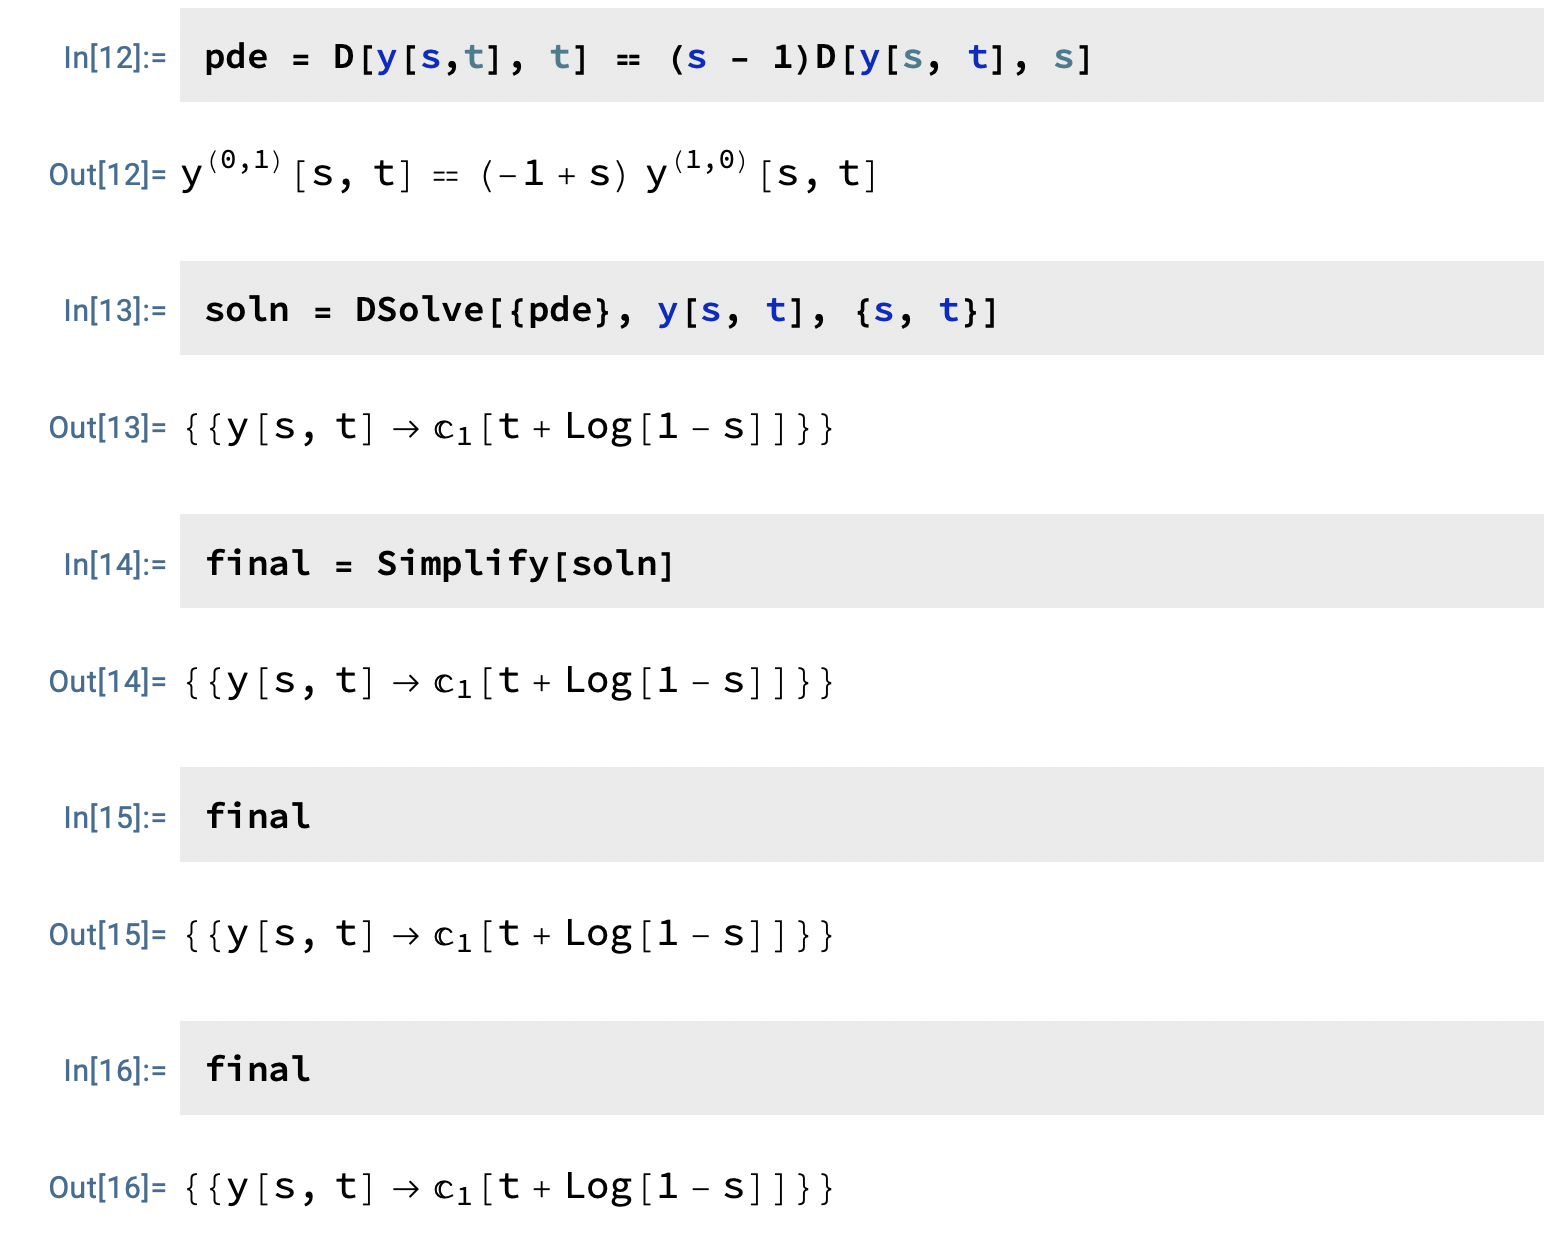
\includegraphics[scale=0.25]{mathematica.png}
	\caption{
		A screen shot of me trying to use mathematica.
	}\label{fig:f1}
\end{figure}
However, with a quick check by hand I think this is off by a sign or something so I am going to move forward with the following
$$
G_{X_t}(s,t) = C(t + \log(s - 1)).
$$
\qed \\

\noindent
{\bf (c)} Find the mean and variance of the process, $E[X(t)]$ and ${\rm Var}(X(t))$. \\

\noindent
\textit{Solution:}
I am not confident in the solution to the PDE that I arrived at, however I am confident that the next steps I take are the correct steps and would provide me the right solutions if the previous part was completed correctly.
I will calculate the mean and variance as follows
$$
E[X(t)] = \frac {\partial}{\partial s}G_{X_t}(1, t) \quad \text{ and } \quad {\rm Var}(X(t)) = \frac {\partial^2}{\partial s^2}G_{X_t}(1, t) + \frac {\partial}{\partial s}G_{X_t}(1, t) - \Big(\frac {\partial}{\partial s}G_{X_t}(1, t)\Big)^2.
$$
Finally let's actually calculate them
\begin{align*}
E[X(t)] &= \frac {\partial}{\partial s}G_{X_t}(1, t) \\
	&= \frac {\partial}{\partial s} C(t + \log(s - 1)) \Big|_{s=1} \\
	&= C\frac 1 {s -1} \Big|_{s=1} \\
	&= C\frac 1 {0}.
\end{align*}
Well obviously this is impossible so I have more evidence that my PDE solution was wrong but I am just done at this point, sorry.
Next to calculate the variance we have
\begin{align*}
{\rm Var}(X(t)) &= \frac {\partial^2}{\partial s^2}G_{X_t}(1, t) + \frac {\partial}{\partial s}G_{X_t}(1, t) - \Big(\frac {\partial}{\partial s}G_{X_t}(1, t)\Big)^2 \\
	&= \frac {\partial^2}{\partial s^2}C(t + \log(s - 1)) \Big|_{s=1} + C\frac 1 {0} + \Big(C\frac 1 {0}\Big)^2 \\
	&= \frac {\partial}{\partial s}C\frac 1 {s - 1} \Big|_{s=1} + C\frac 1 {0} + \Big(C\frac 1 {0}\Big)^2 \\
	&= - C \frac 1 {(s - 1)^2} \Big|_{s=1} + C\frac 1 {0} + \Big(C\frac 1 {0}\Big)^2 \\
	&= - C \frac 1 {0^2} + C\frac 1 {0} + \Big(C\frac 1 {0}\Big)^2.
\end{align*}
Surprise, surprise, I had to divide by zero again multiple times, this is obviously very wrong and I'm still feeling pretty dumb.
\qed \\

\noindent
{\bf (d)} How do the mean and variance of the process compare? Which one will be larger for large time $t$? \\

\noindent
\textit{Solution:} \\
It's virtually impossible for me to comment on this seeing that I have been unsuccessful in every attempt to calculate the mean and variance of this process.
Speculatively speaking I think that the mean would blow up for large $t$ since the rate at which new resistant bacteria show up is proportional to the number of resistant bacteria currently present.
However, further speculation tells me that the variance would be large generally but be overtaken (meaning eventually the mean will be larger than the variance) by the mean due to the previous observation.
\qed \\

\noindent
There is a concluding note for the grader on the next page.

Note: if you need to evaluate a function $f(y)$ at a value $y=y_0$ where it is not defined, you can instead evaluate $\lim_{y\to y_0} f(y)$. \\

\noindent
\textbf{Hi Ruibo, thanks for an excellent course. It was definitely challenging. This exam especially was in a format that made me quite uncomfortable. I realized how heavily I relied on my classmates throughout the quarter and am now exposed to how poorly I understand some of the material. \\ \\ \noindent Or perhaps this is my mind fried at the end of finals week. Nevertheless I know I haven't done very well on this exam. My only hope at the moment is to receive something in the ball park of a 50\%. I also have no idea if this class is scaled in any abnormal manner but I have spent a lot of time stressing out about this as I try to complete this exam. All I want to do is get passing credit for the course to count towards my degree, it doesn't have to be pretty. \\ \\ \noindent Thanks again for all you do and all the help you offered over the course of the quarter. I suppose this is my plea to just at least get passing credit in this class. I know I won't be in the average let alone the top grades, but I don't need that I just want to pass. Thanks for reading my plea or at least letting me get my stresses and thoughts out on paper (LaTeX). Have a great break!}

\end{document}  
